%Reneeth @BS17B025
%To create a pdf with the python environment

\documentclass{article}
\usepackage[utf8]{inputenc}
\usepackage[T1]{fontenc}
\usepackage[utf8]{inputenc}
\usepackage{lmodern}
\usepackage[a4paper, margin=1in]{geometry}

\usepackage{hyperref}
\hypersetup{
    colorlinks=true,
    linkcolor=black,
    filecolor=magenta,      
    urlcolor=green,
}

\usepackage[dvipsnames]{xcolor}
\definecolor{green}{RGB}{0,128,0}
\definecolor{teal}{RGB}{0,128,128}
\definecolor{limegreen}{RGB}{200, 130, 110}
\definecolor{cyan}{RGB}{150,200,210}


\renewcommand{\thesection}{\Roman{section}}


\usepackage{minted}
\large
\title{Programming Assignment 1}

%%%%%%%%%%%%%%%%%%%%%%%%%%%%%%%%%%%%%%%%%%%%%%%%%%%%%%%%%%%%%%%%%%%%%%%%%%%%%%%%%%%%%%%%%%%%%

\begin{document}
\begin{titlepage}
	\begin{center}
    \line(1,0){300}\\
    [0.65cm]
	\huge{\bfseries Programming Assignment I}\\
	\line(1,0){300}\\
	\textsc{\Large CS5691: Pattern Recognition and Machine Learning}\\
	\textsc{\large{Team 17 CCS Section Spring 2021}}\\
	\textsc{ \small{\today}}\\
	[5.5cm]     
	\end{center}
	\begin{flushright}
		\textsc{\Large Aanand Krishnan\\\small{BE17B001}}\\
		[0.5cm]
		\textsc{\Large Manoranjan J\\ \small{NA17B112}}\\
		[0.5cm]
		\textsc{\Large Reneeth Krishna MG\\\small{BS17B025}}
	\end{flushright}
\end{titlepage}
\tableofcontents
\newpage


\section{Linear Regression for Univariate Data}

The Basis Function takes the form,

\begin{equation*}
    \phi{(\mathbf{x})} = {\mathbf{x}^j} \tag{ $0 \leq j \leq Degree$}
\end{equation*}

\subsection{Results of change in regularisation parameter and degree of fit for training data =10}


Generally at lower degrees, the function does not well fit as can be observed from the plots [\ref{fig:1}]. For Degree 6 the function seems to fit well. On the contrary, for degree $9$, it overfits in the case of no regularisation constant. This can be explained by the less number of samples used in the training set and the degree being high. Once the regularisation constant is increased, it fits well till a certain point.

\newpage
\begin{figure}[!ht]
    \centering
    \begin{subfigure}[t]{0.25\textwidth}
        \centering
        \includegraphics[height=1.5in]{Task 1 Images/Batch 10/Figure_1.png}
    \end{subfigure}%
    ~ 
    \begin{subfigure}[t]{0.25\textwidth}
        \centering
        \includegraphics[height=1.5in]{Task 1 Images/Batch 10/Figure_2.png}
    \end{subfigure}%
    ~
    \begin{subfigure}[t]{0.25\textwidth}
        \centering
        \includegraphics[height=1.5in]{Task 1 Images/Batch 10/Figure_3.png}
    \end{subfigure}%
    ~ 
    \begin{subfigure}[t]{0.25\textwidth}
        \centering
        \includegraphics[height=1.5in]{Task 1 Images/Batch 10/Figure_4.png}
    \end{subfigure}%
    \caption{Plots of Polynomials having various orders of degree for a fixed regularisation parameter $\lambda = 0$ using batch size=10}
    \label{fig:1}
\end{figure}


{\rowcolors{3}{green!40!yellow!10}{green!0!yellow!30}
\begin{table}[!ht]
\begin{tabular}{ |p{1.5cm}|p{3cm}|p{3cm}| p{3cm}|  }
\hline
\multicolumn{4}{|c|}{$\mathbf{E}_{rms}$ values for different degrees } \\
\hline
\rowcolor{lightgray} \textbf{Degree} & $\mathbf{E}_{rms-train}$ & $\mathbf{E}_{rms-test}$ & $\mathbf{E}_{rms-valid}$ \\
2   &   1.38  &  1.83   &  2.00   \\   
\hline
 3   &  0.99 &  1.74  &  1.39   \\   
 \hline
 6   &   0.01   &   0.24   &   0.10         \\
 \hline
 9   &   5.4e-4   &    0.19        &     0.42     \\
 \hline
\end{tabular}
\caption{Error comparisons for varying degrees of $\phi(\mathbf{x}) $ for Dataset 1 using batch size=10}
\label{table:1}
\end{table}
}


Since degree 9 is overfit, we experiment with different regularisation parameter lambda the of quadratic regularisation term to see how it affects the fit. For lambda=0.001 and 0.01, the validation Erms decreases than what was before and from 0.1 it increases again. For higher values of lambda the fit is not proper as can be seen from the figures below[\ref{fig:2}].

\newpage
\begin{figure}[!ht]
    \centering
    \begin{subfigure}[ht]{0.5\textwidth}
        \centering
        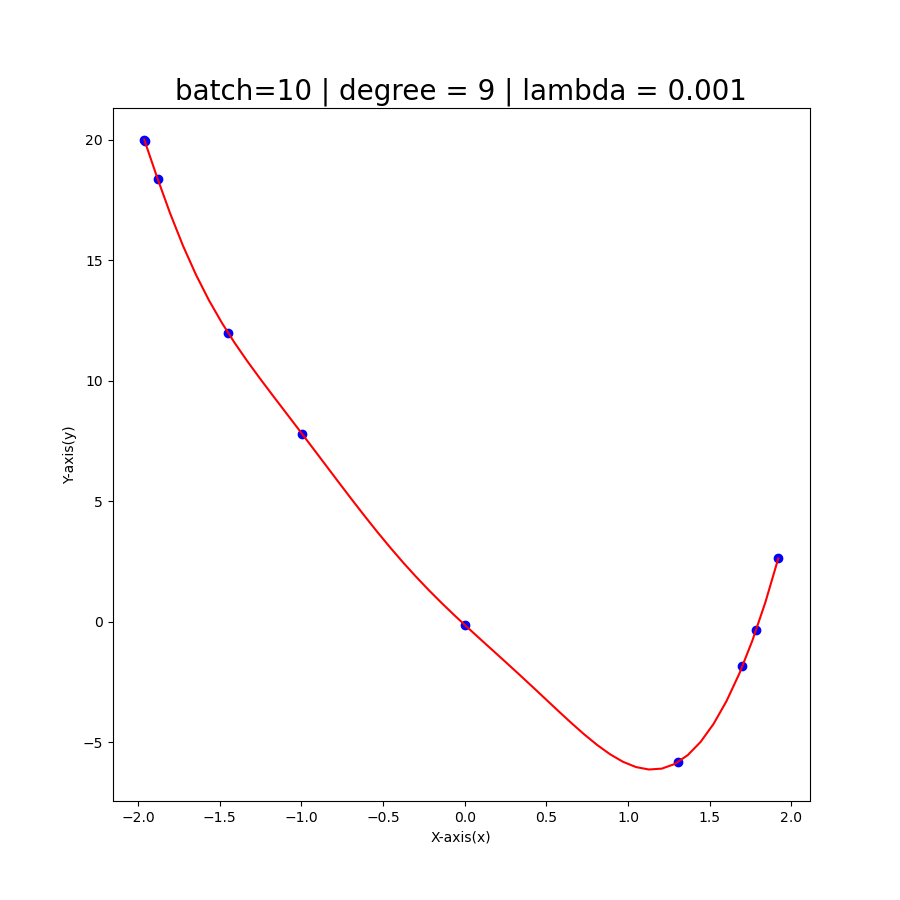
\includegraphics[height=2in]{Task 1 Images/Batch 10/Figure_5.png}
    \end{subfigure}%
    ~ 
    \begin{subfigure}[ht]{0.5\textwidth}
        \centering
        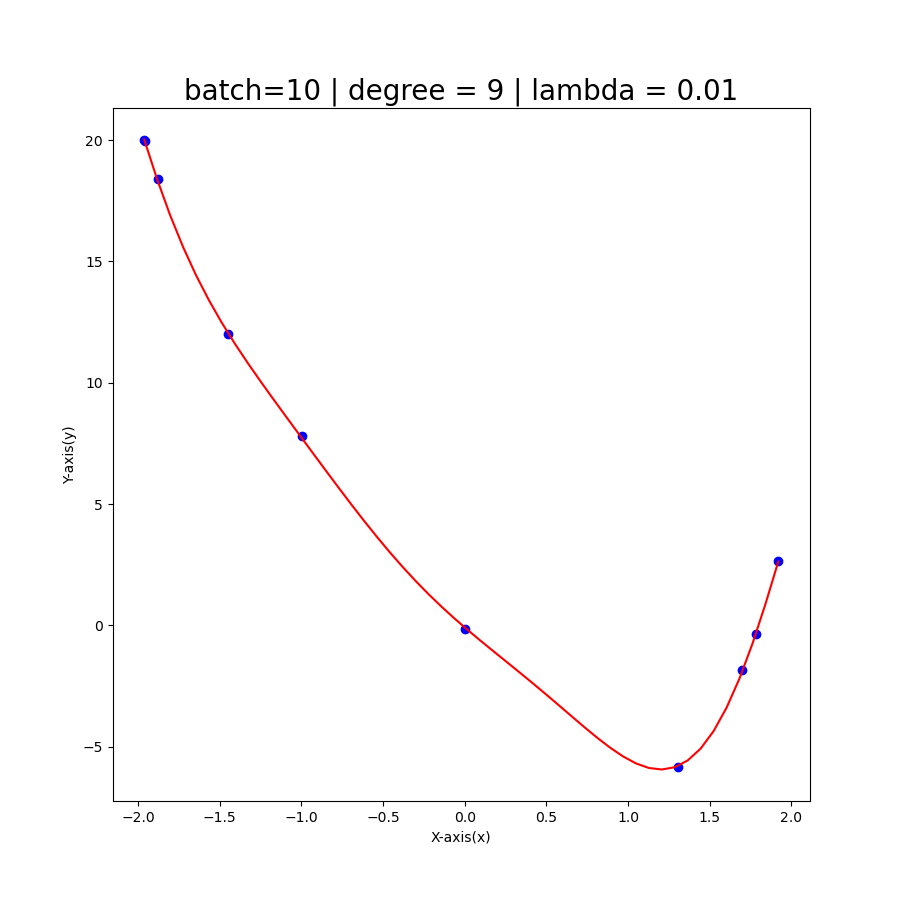
\includegraphics[height=2in]{Task 1 Images/Batch 10/Figure_6.png}
    \end{subfigure}%
    ~
    
    \begin{subfigure}[ht]{0.5\textwidth}
        \centering
        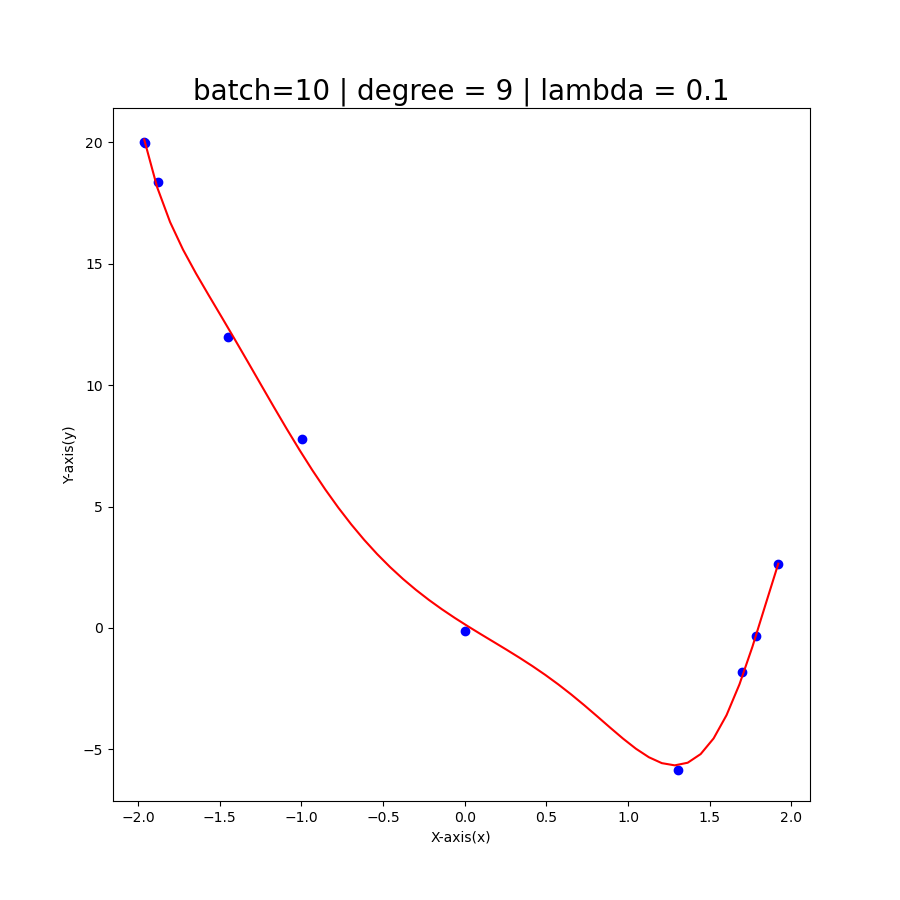
\includegraphics[height=2in]{Task 1 Images/Batch 10/Figure_7.png}
    \end{subfigure}%
    ~ 
    \begin{subfigure}[ht]{0.5\textwidth}
        \centering
        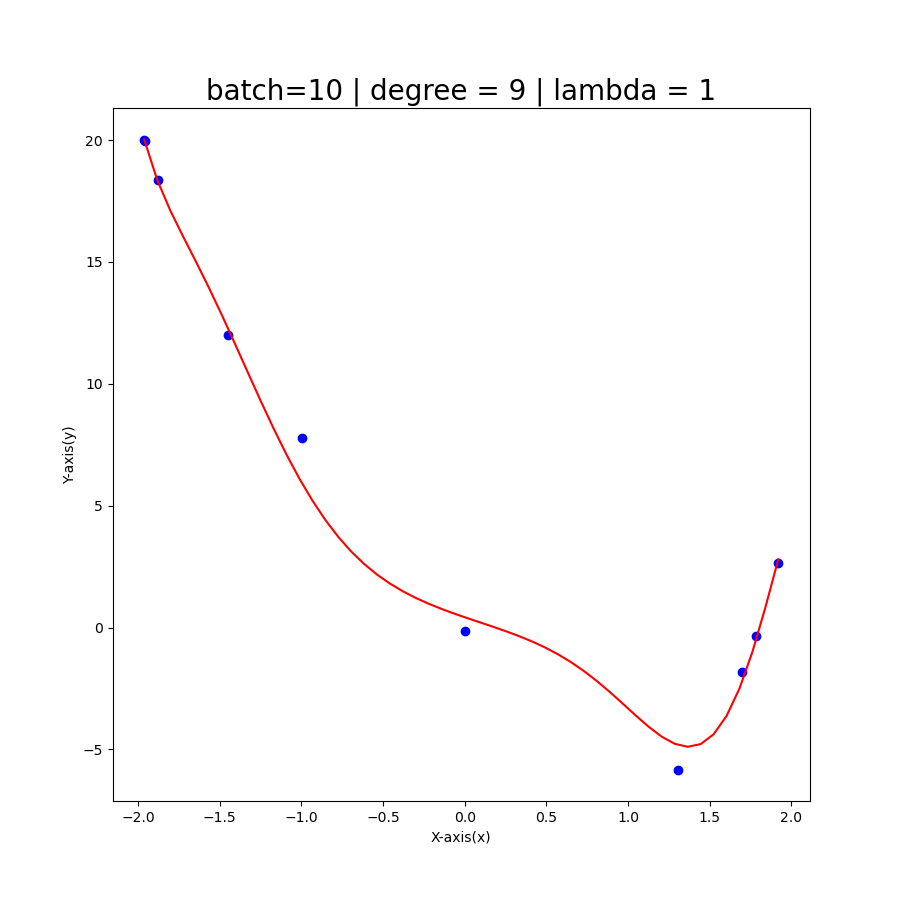
\includegraphics[height=2in]{Task 1 Images/Batch 10/Figure_8.png}
    \end{subfigure}%
    
\end{figure}

\begin{figure}[!ht]
    \centering
    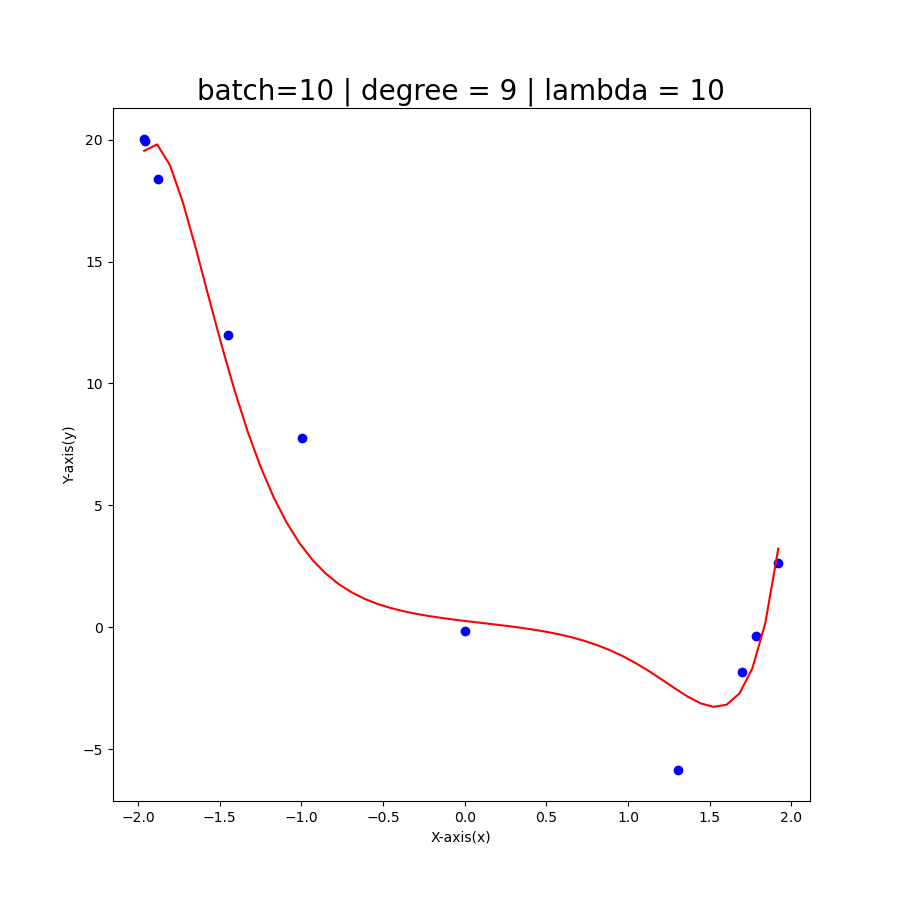
\includegraphics[height=2in]{Task 1 Images/Batch 10/Figure_9.png}
    \caption{Plots of degree 9 Polynomials having various orders of regularisation parameter using batch size=10}
    \label{fig:2}
\end{figure}

{\rowcolors{3}{green!40!yellow!10}{green!0!yellow!30}
\begin{table}[!ht]
\begin{tabular}{ |p{1.5cm}|p{3cm}|p{3cm}| p{3cm}|  }
\hline
\multicolumn{4}{|c|}{$\mathbf{E}_{rms}$ values for different regularisation parameters } \\
\hline
\rowcolor{lightgray} \textbf{lambda} & $\mathbf{E}_{rms-train}$ & $\mathbf{E}_{rms-test}$ & $\mathbf{E}_{rms-valid}$ \\
0.001   &   0.01  &  0.16   &  0.14   \\   
\hline
 0.01   &  0.05 &  0.09  &  0.21   \\   
 \hline
 0.1   &   0.28   &   0.20   &   0.45         \\
 \hline
 1   &   0.71   &    0.41        &     1.15     \\
 \hline
  10   &   1.91   &    0.64        &     2.57     \\
 \hline
\end{tabular}
\caption{Error comparisons for various regularisation parameters with degree=9 for Dataset 1 using batch size=10}
\label{table:2}
\end{table}
}


\subsection{Results for change in regularisation parameter and degree of fit for training data = 200}
Generally at lower degrees, the function does not well fit as can be observed from the plots [\ref{fig:3}]. The fit for degree 6 & 9 seems to be good. Since the validation accuracy is good and the model doesn't seem to overfit, regularisation experiment is not done here.


\begin{figure}[!ht]
    \centering
    \begin{subfigure}[t]{0.25\textwidth}
        \centering
        \includegraphics[height=1.5in]{Task 1 Images/Batch 200/Figure_1.png}
    \end{subfigure}%
    ~ 
    \begin{subfigure}[t]{0.25\textwidth}
        \centering
        \includegraphics[height=1.5in]{Task 1 Images/Batch 200/Figure_2.png}
    \end{subfigure}%
    ~
    \begin{subfigure}[t]{0.25\textwidth}
        \centering
        \includegraphics[height=1.5in]{Task 1 Images/Batch 200/Figure_3.png}
    \end{subfigure}%
    ~ 
    \begin{subfigure}[t]{0.25\textwidth}
        \centering
        \includegraphics[height=1.5in]{Task 1 Images/Batch 200/Figure_4.png}
    \end{subfigure}%
    \caption{Plots of Polynomials having various orders of degree for a fixed regularisation parameter $\lambda = 0$ using batch size200}
    \label{fig:3}
\end{figure}




{\rowcolors{3}{green!40!yellow!10}{green!0!yellow!30}
\begin{table}[!ht]
\begin{tabular}{ |p{1.5cm}|p{3cm}|p{3cm}| p{3cm}|  }
\hline
\multicolumn{4}{|c|}{$\mathbf{E}_{rms}$ values for different degrees } \\
\hline
\rowcolor{lightgray} \textbf{Degree} & $\mathbf{E}_{rms-train}$ & $\mathbf{E}_{rms-test}$ & $\mathbf{E}_{rms-valid}$ \\
2   &   1.64  &  1.73   &  1.70   \\   
\hline
 3   &  1.05 &  0.85  &  1.07   \\   
 \hline
 6   &   0.09   &   0.09   &   0.11         \\
 \hline
 9   &  0.09   &    0.09        &     0.11     \\
 \hline
\end{tabular}
\caption{Error comparisons for varying degrees of $\phi(\mathbf{x}) $ for Dataset 1 using batch size=200}
\label{table:3}
\end{table}
}

\newpage

\section{Linear Regression for Bivariate Data}

The Polynomial Basis Function used takes the form,

\begin{align*}
    \phi{(\mathbf{x})} &= \{\mathbf{x}_1^i \mathbf{x}_2^j\}
    \intertext{Where, $0 \leq i,j \leq Degree$ and $i+j \leq Degree$ In case of data points with two features, the polynomial basis functions includes,}
    \phi{(\mathbf{x})} &= \{ 1,\mathbf{x}_1, \mathbf{x}_2, \mathbf{x}_1^2, \mathbf{x}_2^2, \mathbf{x}_1\mathbf{x}_2, \mathbf{x}_1^{2}\mathbf{x}_1^{2} \}
\end{align*}


\subsection{Experiments $\And$ Observations on Dataset 2: }

\subsubsection{RMS comparison for varying regularisation parameter $\lambda$ (quadratic regularisation):}

Different $\lambda$ values were tested across different models with the goal of finding any $\lambda$ value that might be able to ameliorate any overfitting. However across all models, the increase of $\lambda$ value was accompanied with the strict increase of RMS value. Therefore, subsequent analysis has been carried out without regularization. The best model which was found to be of $batch = 500$ and $degree = 6$ with no regularisation performed with significant accuracy on the training, test and cross validation without any instances of overfitting. The effect of $\lambda$ is illustrated in the figure[\ref{fig:11}]. The table[\ref{table:3}] illustrates the analysis of different $\lambda$ values across the $degree= 6$ model and it can be inferred without doubt from the table that the best fitting model has $\lambda = 0$.

{\rowcolors{3}{green!40!yellow!10}{green!0!yellow!30}
\begin{table}[!ht]
\centering
\scalebox{0.80}{\begin{tabular}{ |p{1.0cm}|p{3.5cm}|p{3.5cm}| p{3.5cm}|  }
\hline
\multicolumn{4}{|c|}{$\mathbf{E}_{rms}$ values for different data } \\
\hline
\rowcolor{lightgray} \textbf{$\lambda$} & $\mathbf{E}_{rms-train}$ & $\mathbf{E}_{rms-test}$ & $\mathbf{E}_{rms-valid}$ \\
\hline
 1   &   7.58e-06  &  1.06e-05   &  7.51e-06   \\   
 \hline
 0   &   1.21e-07   &   1.15e-07  &   1.17e-07         \\
 \hline
 0.1   &   7.75e-06   &    1.06e-06     &     7.77e-07     \\
 \hline
 0.01  &   1.04e-07    &    1.31e-07   &     1.01e-07    \\
 \hline
 0.001  &   1.18e-07  &    1.08-07       &     1.17e-07      \\
 \hline
 0.0001  &   3.30e-08     &     3.2e-08      &      3.08e-08   \\
 \hline
 1e-05   &   1.77e-07    &     1.65e-07      &     1.69e-07  \\
\hline
\end{tabular}}
\caption{Error comparisons for varying values of $\lambda $ for Dataset 2 and a model of $degree = 6$}.
\label{table:4}
\end{table}
}


\begin{figure}[!ht]
    \centering
    \begin{subfigure}[t]{0.25\textwidth}
        \centering
        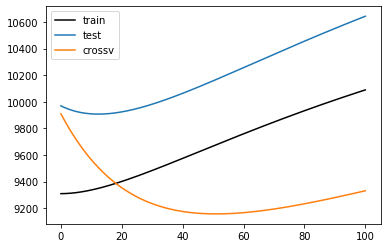
\includegraphics[height=1in]{Task 2 Images/batch500_deg2_lambda.png}
        \caption{Degree, $M = 2$}
    \end{subfigure}%
    ~ 
    \begin{subfigure}[t]{0.25\textwidth}
        \centering
        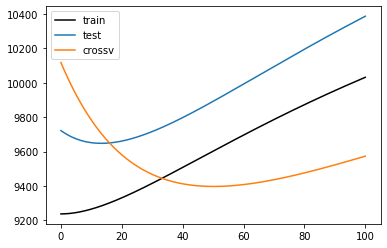
\includegraphics[height=1in]{Task 2 Images/batch500_deg3_lambda.png}
        \caption{Degree, $M = 3$ }
    \end{subfigure}%
    ~
    \begin{subfigure}[t]{0.25\textwidth}
        \centering
        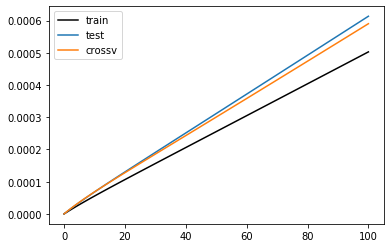
\includegraphics[height=1in]{Task 2 Images/batch500_deg6_lambda1to100.png}
        \caption{ Degree, $M = 6$}
    \end{subfigure}
    \caption{Effect of $\lambda$}
    \label{fig:11}
\end{figure}





\subsubsection{RMS comparison across different models}

Tables [\ref{table:5}], [\ref{table:6}], [\ref{table:7}], and [\ref{table:8}] provides an error based analysis of the model implemented.

{\rowcolors{3}{green!40!yellow!10}{green!0!yellow!30}
\begin{table}[!h]
\begin{tabular}{ |p{1.5cm}|p{3cm}|p{3cm}| p{3cm}|  }
\hline
\multicolumn{4}{|c|}{$\mathbf{E}_{rms}$ values for different data } \\
\hline
\rowcolor{lightgray} Degree & $\mathbf{E}_{rms-train}$ & $\mathbf{E}_{rms-test}$ & $\mathbf{E}_{rms-valid}$ \\
\hline
 2   &   8472.09  &  7916.24  &  11603.31   \\   
 \hline
 3   &   7746.87   &   10209.22  &   9055.03   \\
 \hline
 6   &   1.11e-06   &    7.12e-06     &     1.032e-06    \\
\hline
\end{tabular}
\caption{Error comparisons for varying degrees $\phi(\mathbf{x}) $ for Dataset 2 using 50 samples}.
\label{table:5}
\end{table}

\begin{table}[!h]
 \vspace*{\floatsep}
 \begin{tabular}{ |p{1.5cm}|p{3cm}|p{3cm}| p{3cm}|  }
\hline
\multicolumn{4}{|c|}{$\mathbf{E}_{rms}$ values for different data } \\
\hline
\rowcolor{lightgray} Degree & $\mathbf{E}_{rms-train}$ & $\mathbf{E}_{rms-test}$ & $\mathbf{E}_{rms-valid}$ \\
\hline
 2   &   7836.93  &  9102.67 &  10203.59  \\   
 \hline
 3   &   7410.93  &   8955.31 &   9615.30    \\
 \hline
 6   &   9.07e-08   &    1.14e-07     &     9.06e-08    \\
\hline
\end{tabular}
\caption{Error comparisons for varying degrees $\phi(\mathbf{x}) $ for Dataset 2 using 100 samples}.
\label{table:6}
\end{table}

\begin{table}[!h]
\vspace*{\floatsep}
 \begin{tabular}{ |p{1.5cm}|p{3cm}|p{3cm}| p{3cm}|  }
\hline
\multicolumn{4}{|c|}{$\mathbf{E}_{rms}$ values for different data } \\
\hline
\rowcolor{lightgray} Degree & $\mathbf{E}_{rms-train}$ & $\mathbf{E}_{rms-test}$ & $\mathbf{E}_{rms-valid}$ \\
\hline
 2   &   9007.85  &  9941.50 & 7712.90   \\   
 \hline
 3   &   8891.04   &   10448.97  &   7669.04    \\
 \hline
 6   &   2.77e-08   &    3.15e-08     &     3.17e-08   \\
\hline
\end{tabular}
\caption{Error comparisons for varying degrees $\phi(\mathbf{x}) $ for Dataset 2 using 200 samples}.
\label{table:7}
\end{table}

\begin{table}[!ht]
\vspace*{\floatsep}
 \begin{tabular}{ |p{1.5cm}|p{3cm}|p{3cm}| p{3cm}|  }
\hline
\multicolumn{4}{|c|}{$\mathbf{E}_{rms}$ values for different data } \\
\hline
\rowcolor{lightgray} Degree & $\mathbf{E}_{rms-train}$ & $\mathbf{E}_{rms-test}$ & $\mathbf{E}_{rms-valid}$ \\
\hline
 2   &   9308.74  &  9968.55 & 9908.81   \\   
 \hline
 3   &   9237.93   &   9721.98  &   10117.44    \\
 \hline
 6   &   2.54e-08   &    2.92e-08     &     2.51e-08  \\
\hline
\end{tabular}
\caption{Error comparisons for varying degrees $\phi(\mathbf{x}) $ for Dataset 2 using 500 samples}.
\label{table:8}
\end{table}
}


\newpage
\subsubsection{Surface Plots with Training set superimposed}
Figures [\ref{fig:12}], [\ref{fig:13}], [\ref{fig:14}] and [\ref{fig:15}] are the various surface plots.

\begin{figure}[!ht]
    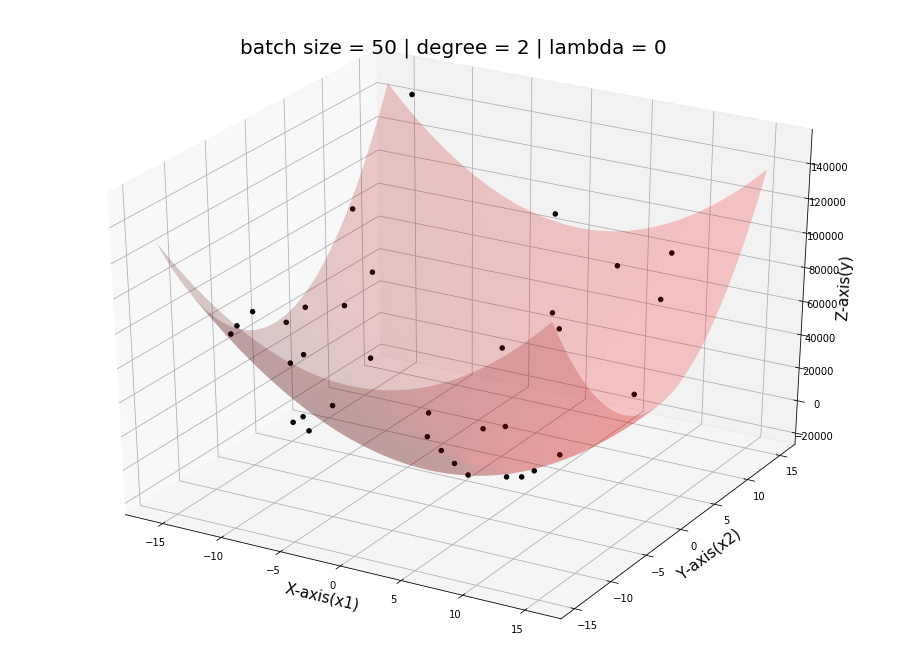
\includegraphics[width=.30\textwidth]{Task 2 Images/surfaceplot_batch50_deg2_lamb0.png}\hfill
    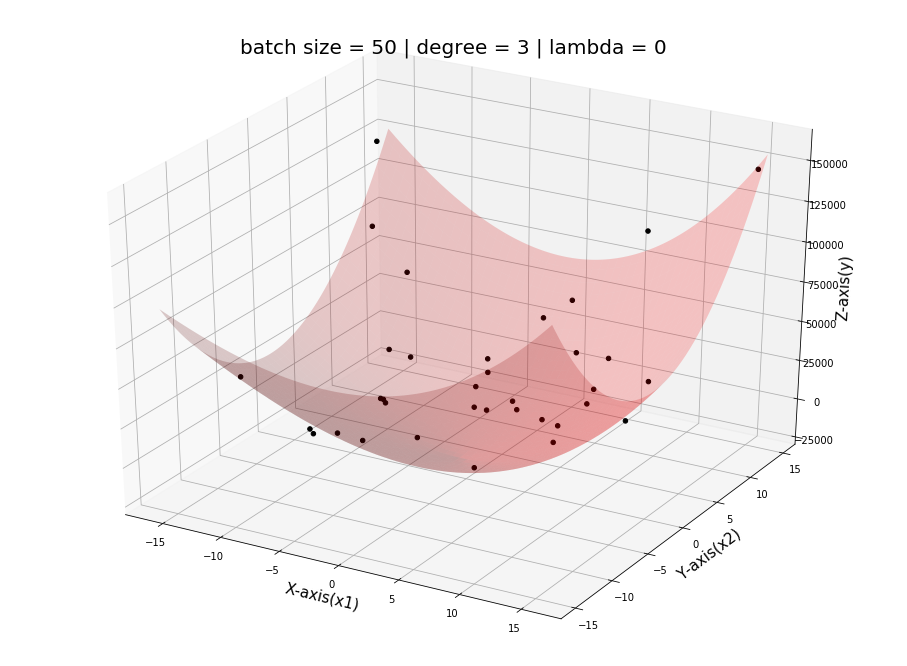
\includegraphics[width=.30\textwidth]{Task 2 Images/surfaceplot_batch50_deg3_lamb0.png}\hfill
    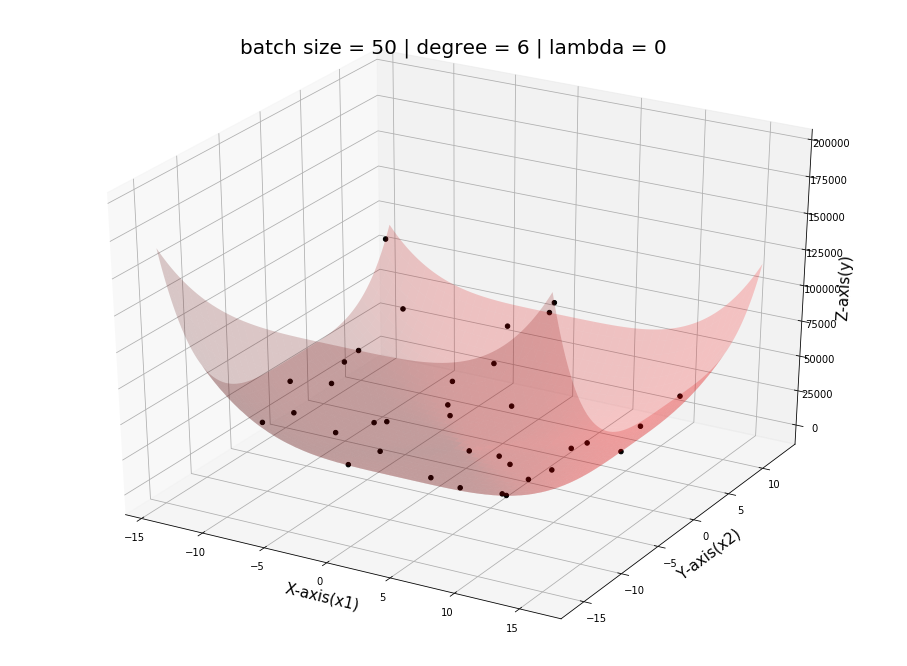
\includegraphics[width=.30\textwidth]{Task 2 Images/surfaceplot_batch50_deg6_lamb0.png}
    \caption{Surface Plots using various degree for a fixed best regularisation parameter $\lambda = 0$ using 50 samples }
    \label{fig:12}
\end{figure}

\begin{figure}[!ht]
    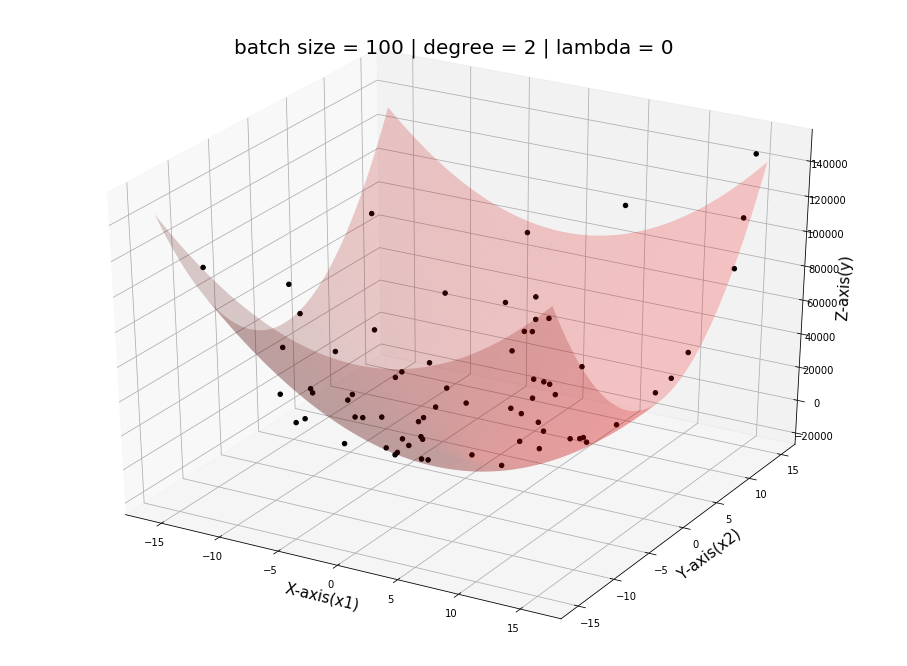
\includegraphics[width=.30\textwidth]{Task 2 Images/surfaceplot_batch100_deg2_lamb0.png}\hfill
    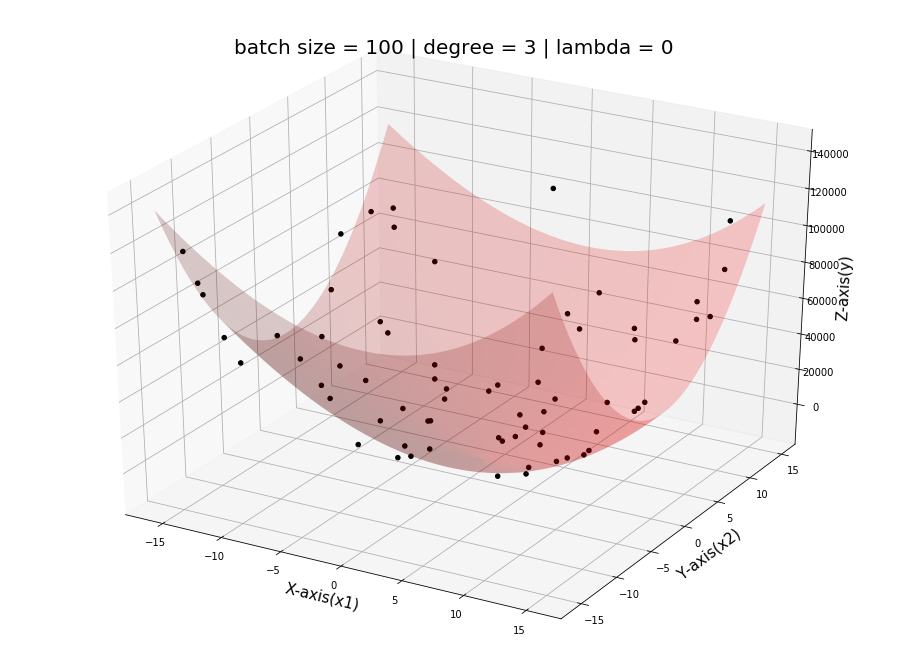
\includegraphics[width=.30\textwidth]{Task 2 Images/surfaceplot_batch100_deg3_lamb0.png}\hfill
    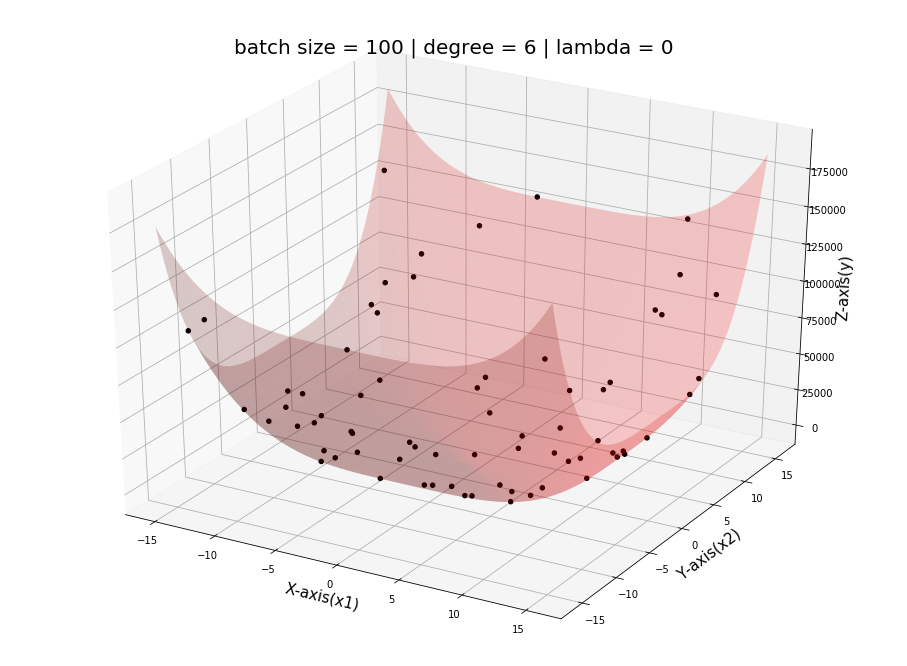
\includegraphics[width=.30\textwidth]{Task 2 Images/surfaceplot_batch100_deg6_lamb0.png}
    \caption{Surface Plots using various degree for a fixed regularisation parameter $\lambda = 0$ using 100 samples}
    \label{fig:13}
\end{figure}

\begin{figure}[!ht]
    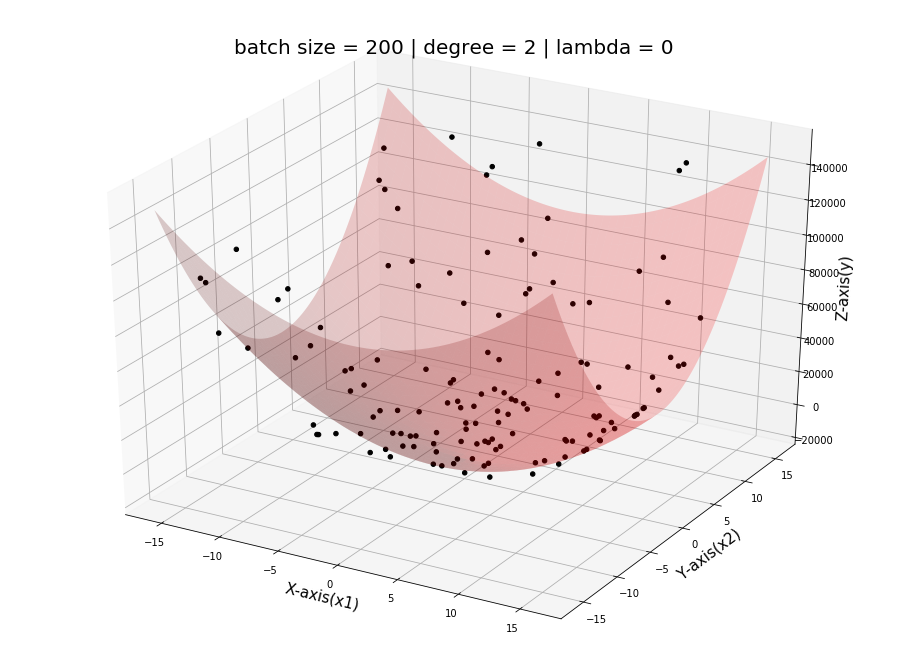
\includegraphics[width=.30\textwidth]{Task 2 Images/surfaceplot_batch200_deg2_lamb0.png}\hfill
    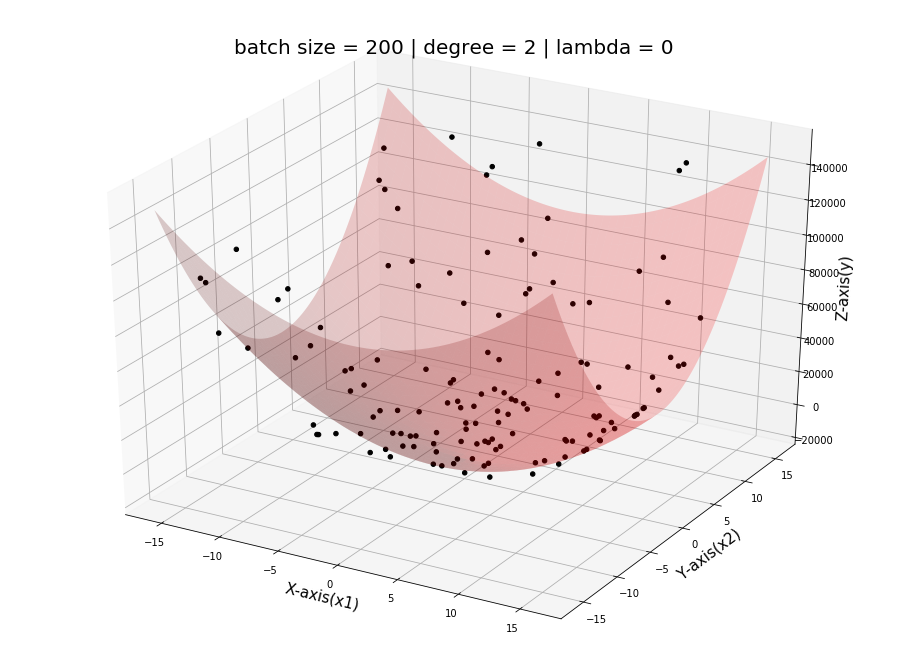
\includegraphics[width=.30\textwidth]{Task 2 Images/surfaceplot_batch200_deg2_lamb0.png}\hfill
    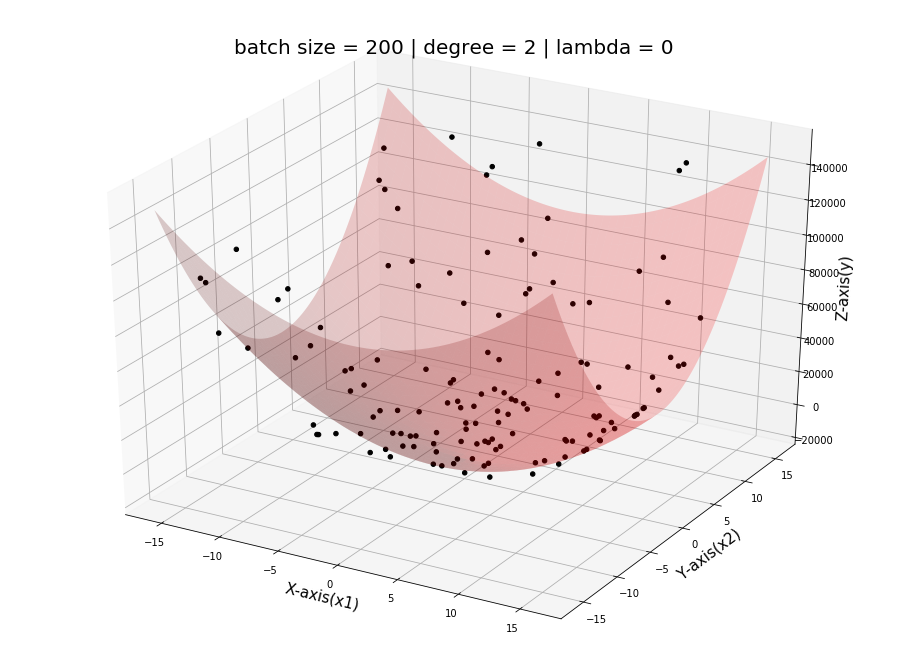
\includegraphics[width=.30\textwidth]{Task 2 Images/surfaceplot_batch200_deg2_lamb0.png}
    \caption{Surface Plots using various degree for a fixed regularisation parameter $\lambda = 0$ using 200 samples}
    \label{fig:14}
 \end{figure}


\begin{figure}[!ht] 
    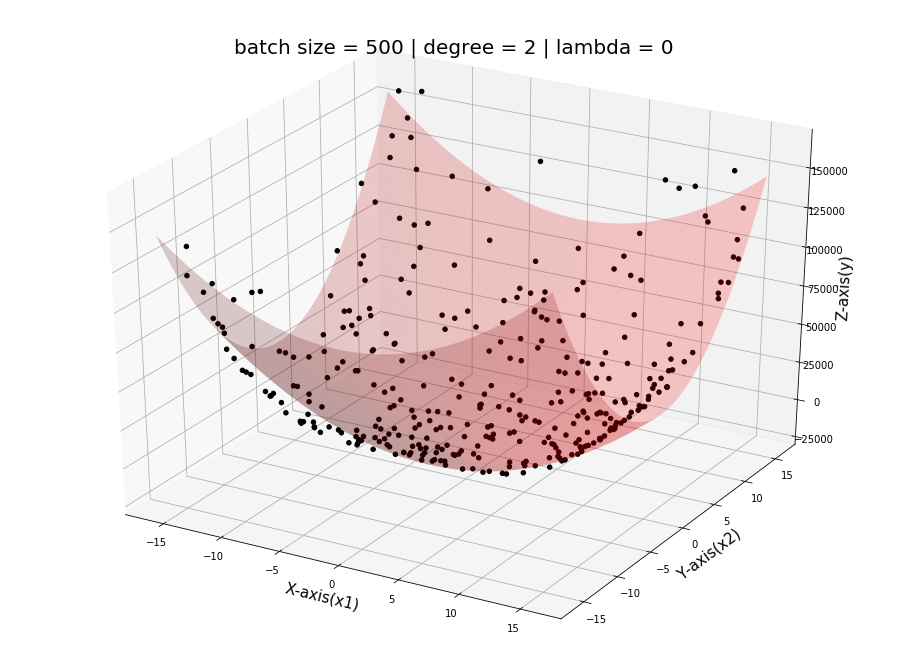
\includegraphics[width=.30\textwidth]{Task 2 Images/surfaceplot_batch500_deg2_lamb0.png}\hfill
    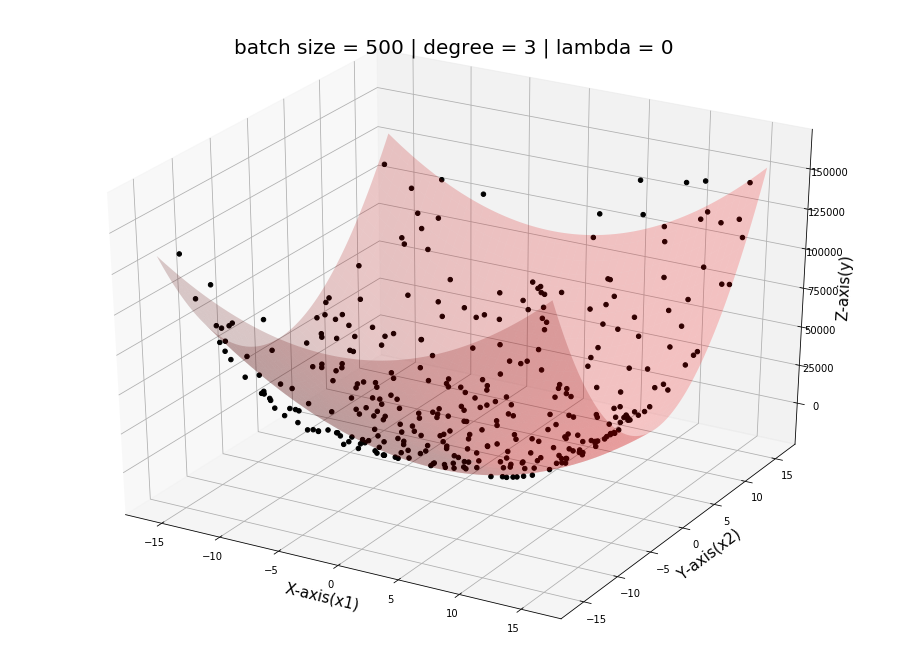
\includegraphics[width=.30\textwidth]{Task 2 Images/surfaceplot_batch500_deg3_lamb0.png}\hfill
    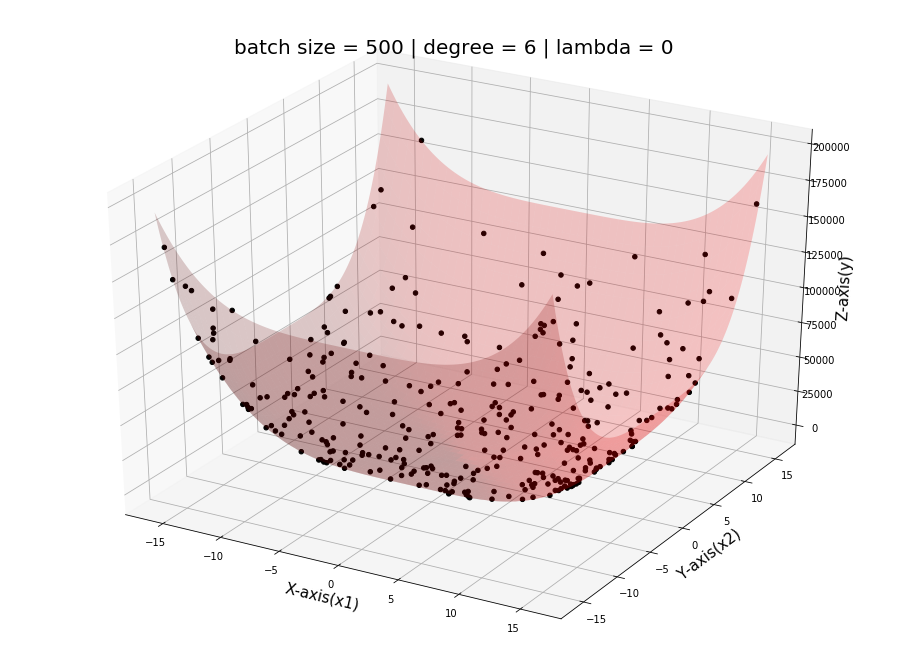
\includegraphics[width=.30\textwidth]{Task 2 Images/surfaceplot_batch500_deg6_lamb0.png}
    \caption{Surface Plots using various degree for a fixed regularisation parameter $\lambda = 0$ using 500 samples}
    \label{fig:15}
\end{figure}

\newpage
\subsubsection{Scatter Plots of the Best Model}
The best model was found to be of batch size 500 and degree 6 without any regularization and fared significantly better than the other degree 2,3 models as it's $E_{rms}$ values were found to be smaller in orders of magnitude $10^9$. Scatter plots of the best model are represented in figure [\ref{fig:16}]


 \begin{figure}[!ht]
     \centering
     \begin{subfigure}[t]{0.30\textwidth}
         \centering
         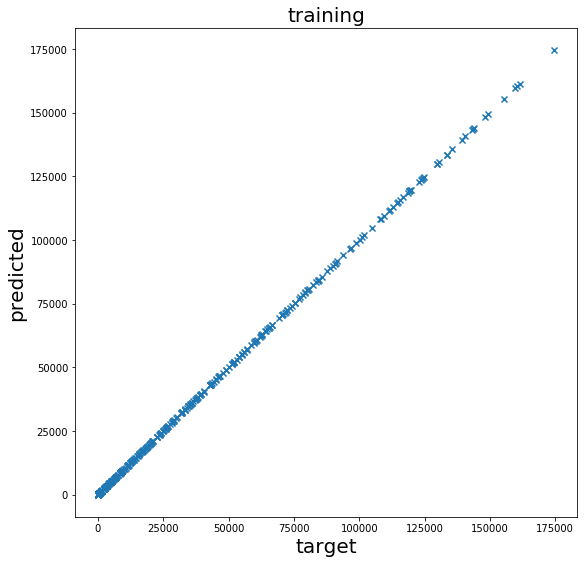
\includegraphics[height=1.6in]{Task 2 Images/best_scatterplot_batch_500_degree_6_lambda_0_training.png}
         \caption{Training Data}
     \end{subfigure}%
     ~ 
     \begin{subfigure}[t]{0.30\textwidth}
         \centering
         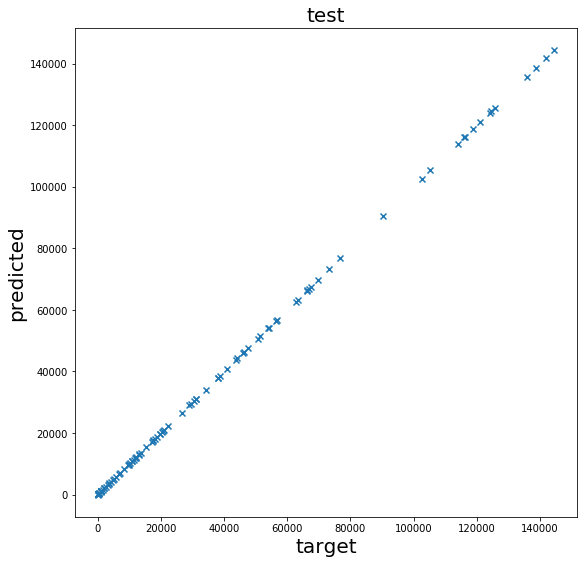
\includegraphics[height=1.6in]{Task 2 Images/best_scatterplot_batch_500_degree_6_lambda_0_test.png}
         \caption{Test Data }
     \end{subfigure}%
     ~
     \begin{subfigure}[t]{0.30\textwidth}
         \centering
         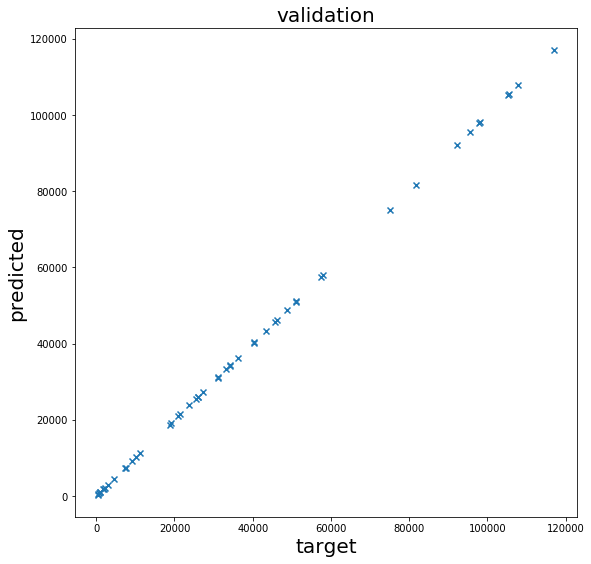
\includegraphics[height=1.6in]{Task 2 Images/best_scatterplot_batch_500_degree_6_lambda_0_validation.png}
         \caption{Validation Data }
     \end{subfigure}
     \caption{Best Scatter Plot}
     \label{fig:16}
\end{figure}


\newpage

\section{Linear Model for Regression using Gaussian Basis Functions}
\subsection{\textcolor{teal}{Python Code}}

\begin{minted}[frame=lines, linenos, fontsize=\large]
{python}

# -*- coding: utf-8 -*-


import numpy as np
import pandas as pd
import matplotlib.pyplot as plt

################################ Dataset 3 ###################################

def process_dataset_3(D, var, r):
    
    """
    D: No of gauss functions for fit
    var: variance for fit
    r: regularisation term
    """
    # Read txt file
    
    f = open('datasets/2_music.txt', 'r')
    
    length = 0
    for line in f:
        
        d = [float(i) for i in line.split(',')]
        
        if length == 0:
            data = np.array(d)
            data = data[np.newaxis,:]
        else:
            d = np.array(d)
            d = d[np.newaxis,:]
            data = np.append(data,d,axis=0)
        length = length+1
    
    f.close()
       
    data = pd.DataFrame(data)
    
    
    # shuffle dataset
    data = data.sample(frac=1)
    
    # get dependent and independent varaible
    data = np.array(data)
    
    
    X = data[:,0:-2]
    y = data[:,-2:]
    
    # get unique values of y
    y_unique = np.unique(y,axis=0)
    
    # length of data for fit
    train_len = int(np.shape(X)[0]*0.7)
    val_len = int(np.shape(X)[0]*0.2)
    test_len = int(np.shape(X)[0]) - val_len - train_len
    
    # test train split
    X_train = X[0:train_len]
    X_test = X[train_len:train_len+test_len]
    X_val = X[train_len+test_len:train_len+test_len+val_len]
    
    y_train = y[0:train_len]
    y_test = y[train_len:train_len+test_len]
    y_val = y[train_len+test_len:train_len+test_len+val_len]
    
    # K-means clustering
    loop = 1
    prev_zni = np.zeros((train_len,D-1))
    
    while(loop>0):
        zni = np.zeros((train_len,D-1))
        
        if loop == 1:
            # randomly choose k points
            random_index = np.random.randint(0,train_len,D-1)
        
            # Initialize MUi
            MUi = X_train[random_index,:]
        
        # Determine points belonging to clusters
        for j in range(0,train_len):
            i = np.argmin(np.linalg.norm(X_train[j,:]-MUi,axis=1),axis=0)
            zni[j,i] = 1
            
        # Determine number of datapoints in the clusters
        Ni = np.sum(zni,axis=0)
        
        # Update MUi
        for j in range(0,D-1):
            if Ni[j] == 0:
                continue
            
            z = zni[:,j]
            MUi[j,:] = (np.sum(X_train*z[:,np.newaxis],axis=0))/Ni[j]
            
        # compare previous and current Zni
        comp = prev_zni - zni
        
        prev_zni = zni
        loop = loop+1
        
        # if no change break the loop
        if np.max(comp) == 0 and np.min(comp) == 0:
            break
    
    # Assign Mui
    mu = MUi
    
    # gaussian function
    phii = lambda x,mu : np.e**(-(np.linalg.norm(x-mu))/var**2)
    
    # Formulate phi matrix for training data
    phin = np.zeros((train_len,D))
    
    for i in range(0,train_len):
        for j in range(0,D):
            if j==0:
                phin[i,j] = 1
                #phin[i,j] = phii(X_train[i,:],mu[j,:])
            else:
                phin[i,j] = phii(X_train[i,:],mu[j,:])
            
    # weights with quadratic regularisation
    W = np.linalg.inv(phin.T@phin + r*np.identity(D))@phin.T@y_train
    
    # weights with tikhanov regularisation
    # phin_bar = np.zeros((D,D))
    # for i in range(0,D):
    #     for j in range(0,D):
    #         phin_bar[i,j] = np.exp(np.linalg.norm(mu[i,:]-mu[j,:])/var**2)
    
    # W = np.linalg.inv(phin.T@phin + r*phin_bar)@phin.T@y_train
    
    ###########################################################################
    
    # Test on training dataset
    y_pred = np.zeros((train_len,2))
    
    # Formulate phi matrix for training data
    phin = np.zeros((train_len,D))
    
    for i in range(0,train_len):
        for j in range(0,D):
            if j==0:
                phin[i,j] = 1
                # phin[i,j] = phii(X_train[i,:],mu[j,:])
            else:
                phin[i,j] = phii(X_train[i,:],mu[j])
    
    for i in range(0,train_len):
        pred = (phin[i,:])@W
        y_pred[i,:] = pred
        
        # term1 = np.deg2rad((pred[0] - y_unique[:,0])/2)
        # term2 = np.deg2rad((pred[1] - y_unique[:,1])/2)
        # a = (np.sin(term1)**2) + # np.cos(np.deg2rad(pred[0]))*
        #      np.cos(np.deg2rad(y_unique[:,0]))*(np.sin(term2# )**2)
        # dist = 2*6373*np.arctan2(np.sqrt(a),np.sqrt(1-a))
        
        # index = np.argmin(dist)
        # y_pred[i,:] = y_unique[index,:]
    
    Erms_train1 = ((np.linalg.norm(y_pred[:,0]-y_train[:,0])))/np.sqrt(train_len)
    Erms_train2 = ((np.linalg.norm(y_pred[:,1]-y_train[:,1])))/np.sqrt(train_len)

    # # scatter plot
    # fig1 = plt.figure(figsize=(9,9))
    # plt.scatter(y_train[:,0],y_pred[:,0],marker='x')
    # plt.scatter(y_train[:,1],y_pred[:,1],marker='x')
    # plt.xlabel('target',fontsize=20)
    # plt.ylabel('predicted',fontsize=20)
    # plt.title("Gaussian Basis Function (For Dataset 3 of # best performing 
    #             model with training data) | degree = {} | # lambda = {}".format(D,r),
    #             fontsize = 20)
    # plt.legend(["y0","y1"])
    ###########################################################################
    
    # Test on validation dataset
    y_pred = np.zeros((val_len,2))
    
    # Formulate phi matrix for validation data
    phin = np.zeros((val_len,D))
    
    for i in range(0,val_len):
        for j in range(0,D):
            if j==0:
                phin[i,j] = 1
                # phin[i,j] = phii(X_val[i,:],mu[j,:])
            else:
                phin[i,j] = phii(X_val[i,:],mu[j])
    
    for i in range(0,val_len):
        pred = (phin[i,:])@W
        y_pred[i,:] = pred
    
    
    Erms_val1 = ((np.linalg.norm(y_pred[:,0]-y_val[:,0])))/np.sqrt(val_len)
    Erms_val2 = ((np.linalg.norm(y_pred[:,1]-y_val[:,1])))/np.sqrt(val_len)
    
    # scatter plot for validation data
    # fig1 = plt.figure(figsize=(9,9))
    # plt.scatter(y_val,y_pred,marker='x')
    # plt.xlabel('target',fontsize=20)
    # plt.ylabel('predicted',fontsize=20)
    # plt.title("Gaussian Basis Function (For Dataset 2 of best performing model 
    #            with validation data) | degree = {} | lambda # = {}".format(D,r),
    #             fontsize = 20)
    
    ###############################################################################
    
    # Test on test dataset
    y_pred = np.zeros((test_len,2))
    
    # Formulate phi matrix for test data
    phin = np.zeros((test_len,D))
    
    for i in range(0,test_len):
        for j in range(0,D):
            if j==0:
                phin[i,j] = 1
                #phin[i,j] = phii(X_test[i,:],mu[j,:])
            else:
                phin[i,j] = phii(X_test[i,:],mu[j])
    
    for i in range(0,test_len):
        pred = (phin[i,:])@W
        y_pred[i,:] = pred
        
    Erms_test1 = ((np.linalg.norm(y_pred[:,0]-y_test[:,0])))/np.sqrt(test_len)
    Erms_test2 = ((np.linalg.norm(y_pred[:,1]-y_test[:,1])))/np.sqrt(test_len)
    
    # scatter plot for test data
    fig1 = plt.figure(figsize=(9,9))
    plt.scatter(y_test[:,0],y_pred[:,0],marker='x')
    plt.scatter(y_test[:,1],y_pred[:,1],marker='x')
    plt.xlabel('target',fontsize=20)
    plt.ylabel('predicted',fontsize=20)
    plt.title("Gaussian Basis Function (For Dataset 3 of best performing model
               with test data) | degree = {} | lambda = {}".format(D,r),
                fontsize = 20)
    plt.legend(["y0","y1"])
    ###########################################################################
    return Erms_train1, Erms_train2, Erms_val1, Erms_val2, Erms_test1, Erms_test2
    
################################ Dataset 2 ###################################

def process_dataset_2(D, var, r):
    
    """
    D: No of gauss functions for fit
    var: variance for fit
    r: regularisation term
    """
    
    # Read csv file
    data = pd.read_csv('datasets/function1_2d.csv')
    
    # shuffle dataset
    # data = data.sample(frac=1)
    
    # get dependent and independent varaible
    X = data[['x1','x2']]
    y = data['y']
    
    # convert into numpy
    X = np.array(X)
    y = np.array(y)
    
    # length of data for fit
    train_len = int(np.shape(X)[0]*0.7)
    test_len = int(np.shape(X)[0]*0.2)
    val_len = int(np.shape(X)[0]*0.1)
    
    # test train split
    X_train = X[0:train_len]
    X_test = X[train_len:train_len+test_len]
    X_val = X[train_len+test_len:train_len+test_len+val_len]
    
    y_train = y[0:train_len]
    y_test = y[train_len:train_len+test_len]
    y_val = y[train_len+test_len: train_len+test_len+val_len]
    
    # K-means clustering
    loop = 1
    prev_zni = np.zeros((train_len,D-1))
    
    while(loop>0):
        zni = np.zeros((train_len,D-1))
        
        if loop == 1:
            # randomly choose k points
            random_index = np.random.randint(0,train_len,D-1)
        
            # Initialize MUi
            MUi = X_train[random_index,:]
        
        # Determine points belonging to clusters
        for j in range(0,train_len):
            i = np.argmin(np.linalg.norm(X_train[j,:]-MUi,axis=1),axis=0)
            zni[j,i] = 1
            
        # Determine number of datapoints in the clusters
        Ni = np.sum(zni,axis=0)
        
        # Update MUi
        for j in range(0,D-1):
            if Ni[j] == 0:
                continue
            
            z = zni[:,j]
            MUi[j,:] = (np.sum(X_train*z[:,np.newaxis],axis=0))/Ni[j]
            
        # compare previous and current Zni
        comp = prev_zni - zni
        
        prev_zni = zni
        loop = loop+1
        
        # if no change break the loop
        if np.max(comp) == 0 and np.min(comp) == 0:
            break
    
    # Assign Mui
    mu = MUi
    
    # gaussian function
    phii = lambda x,mu : np.e**(-(np.linalg.norm(x-mu))/var**2)
    
    # Formulate phi matrix for training data
    phin = np.zeros((train_len,D))
    
    for i in range(0,train_len):
        for j in range(0,D):
            if j==0:
                phin[i,j] = 1
            else:
                phin[i,j] = phii(X_train[i,:],mu[j-1,:])
            
    
    # weights with quadratic regularisation
    W = np.linalg.inv(phin.T@phin + r*np.identity(D))@phin.T@y_train
    
    ###########################################################################
    
    # Test on training dataset
    y_pred = np.zeros((train_len,1))
    
    # Formulate phi matrix for training data
    phin = np.zeros((train_len,D))
    
    for i in range(0,train_len):
        for j in range(0,D):
            if j==0:
                phin[i,j] = 1
            else:
                phin[i,j] = phii(X_train[i,:],mu[j-1])
    
    for i in range(0,train_len):
        y_pred[i,:] = (phin[i,:])@W
        
    Erms_train = ((np.linalg.norm(y_pred-y_train[:,np.newaxis])))/
                   np.sqrt(train_len)
    
    
    # # scatter plot for training data
    # fig1 = plt.figure(figsize=(9,9))
    # plt.scatter(y_train,y_pred,marker='x')
    # plt.xlabel('target',fontsize=20)
    # plt.ylabel('predicted',fontsize=20)
    # plt.title("Gaussian Basis Function (For Dataset 2 of best performing model
    #             with training data) | degree = {} | lambda = # {}".format(D,r),
    #              fontsize = 20)
    
    
    ###########################################################################
    
    # Test on validation dataset
    y_pred = np.zeros((val_len,1))
    
    # Formulate phi matrix for validation data
    phin = np.zeros((val_len,D))
    
    for i in range(0,val_len):
        for j in range(0,D):
            if j==0:
                phin[i,j] = 1
            else:
                phin[i,j] = phii(X_val[i,:],mu[j-1])
    
    for i in range(0,val_len):
        y_pred[i,:] = (phin[i,:])@W
        
    Erms_val = ((np.linalg.norm(y_pred-y_val[:,np.newaxis])))/np.sqrt(val_len)
    
    # scatter plot for validation data
    # fig1 = plt.figure(figsize=(9,9))
    # plt.scatter(y_val,y_pred,marker='x')
    # plt.xlabel('target',fontsize=20)
    # plt.ylabel('predicted',fontsize=20)
    # plt.title("Gaussian Basis Function (For Dataset 2 of best performing model 
    #             with validation data) | degree = {} | lambda #= {}".format(D,r),
    #              fontsize = 20)
    
    ###########################################################################
    
    # Test on test dataset
    y_pred = np.zeros((test_len,1))
    
    # Formulate phi matrix for test data
    phin = np.zeros((test_len,D))
    
    for i in range(0,test_len):
        for j in range(0,D):
            if j==0:
                phin[i,j] = 1
            else:
                phin[i,j] = phii(X_test[i,:],mu[j-1])
    
    for i in range(0,test_len):
        y_pred[i,:] = (phin[i,:])@W
        
    Erms_test = ((np.linalg.norm(y_pred-y_test[:,np.newaxis])))/np.sqrt(test_len)
    
    # # scatter plot for validation data
    # fig1 = plt.figure(figsize=(9,9))
    # plt.scatter(y_test,y_pred,marker='x')
    # plt.xlabel('target',fontsize=20)
    # plt.ylabel('predicted',fontsize=20)
    # plt.title("Gaussian Basis Function (For Dataset 2 of best performing 
    #             model with test data) | degree = {} | lambda # = {}".format(D,r),
    #              fontsize = 20)
    
    ###########################################################################
    return Erms_train, Erms_val, Erms_test
    

############################ Main Code ########################################

# Call function to experiment dataset 2/3
D = [2,3,6,9,20,33,40,100]
var = [1,3,5,10,50,100]
reg = [0,10e-5,10e-4,10e-3,10e-2,10e-1,10,10e2,10e3,10e4,10e5]

Erms = []
# Experiment with variance
for v in var:
    erms = process_dataset_3(100, v, 0)
     Erms.append(erms)
    
# Plot table
fig = plt.figure(figsize=(9,9))
row_labels=["var = 1", "var = 3", "var = 5", "var = 10", "var = 50", "var = 100"]
column_labels=["Erms_train", "Erms_val", "Erms_test"]
column_labels=["Erms_train_y0","Erms_train_y1", "Erms_val0","Erms_val1",
                 "Erms_test0", "Erms_test1"]
plt.axis('tight')
plt.axis('off')
plt.table(cellText=Erms,rowLabels=row_labels,colLabels=column_labels, loc="center")

Erms = []
# Experiment with Dimensions
for d in D:
    erms = process_dataset_3(d, 3, 0)
    Erms.append(erms)

# Plot table
fig = plt.figure(figsize=(9,9))
row_labels=["D = 2", "D = 3", "D = 6", "D = 9", "D = 20", "D = 30",
              "D = 40", "D = 100"]
column_labels=["Erms_train", "Erms_val", "Erms_test"]
column_labels=["Erms_train_y0","Erms_train_y1", "Erms_val0","Erms_val1", 
                 "Erms_test0", "Erms_test1"]
plt.axis('tight')
plt.axis('off')
plt.table(cellText=Erms,rowLabels=row_labels,colLabels=column_labels,
            loc="center")

Erms = []  
# Experiment with regularisation
for r in reg:
    erms = process_dataset_3(100, 3, r)
    Erms.append(erms)
    
# Plot table
fig = plt.figure(figsize=(9,9))
row_labels=["lambda = 0", "lambda = 10e-5", "lambda = 10e-4", "lambda = 10e-3", 
              "lambda = 10e-2", "lambda = 10e-1", "lambda = 10", "lambda = 10e2", 
              "lambda = 10e3", "lambda = 10e4", "lambda = 10e5"]
column_labels=["Erms_train", "Erms_val", "Erms_test"]
column_labels=["Erms_train_y0","Erms_train_y1", "Erms_val0","Erms_val1", 
                 "Erms_test0", "Erms_test1"]
plt.axis('tight')
plt.axis('off')
plt.table(cellText=Erms,rowLabels=row_labels,colLabels=column_labels,
            loc="center")
\end{minted}


%\newpage

\section{Direct links For Python Codes}

\begin{itemize}
    \item \href{https://drive.google.com/file/d/1mxY9pXO8wiZVVD0q3yLTu1v4Fx4q6NzI/view?usp=sharing}{Polynomial Curve Fitting}
    \item \href{https://drive.google.com/file/d/1nWiG9Q4ry0lCtlhq9HL9ZXIbecmPnXi5/view?usp=sharing}{Linear Model for Regression using Polynomial Basis Functions}
    \item \href{https://drive.google.com/file/d/1zqY76i_a3TWYNmjPhV_a--PqXhK_LwDk/view?usp=sharing}{Linear Model for Regression using Gaussian Basis Functions}
\end{itemize}


\end{document}











